\documentclass[10pt, titlepage, oneside, a4paper]{article}
\usepackage{array}
\usepackage{caption}
\usepackage{fancyhdr}
\usepackage{graphicx}
\usepackage{hyperref}
\usepackage{lastpage}
\usepackage{lmodern}
\usepackage[utf8]{inputenc}
\usepackage{polski}

\graphicspath{ {./images/} }
\urlstyle{same}

\title{Specyfikacja Projektu ,,Expert4Home''}
\author{K. Dąbrowski, J. Grygiel, S. Kalisz\\
K. Malinowski, P. Piętka, B.Zdrojewski}
\date{Wersja 1.0\\\today}

\pagestyle{fancy}
\fancyhf{}
\lhead{Specyfikacja Projektu ,,Expert4Home''}
\rhead{Wersja 1.0}
\rfoot{\thepage \hspace{1pt} / \pageref{LastPage}}

\begin{document}

	\maketitle
	\thispagestyle{empty}  
	\newpage
  
	\section{Wstęp} 
  
	\subsection{Cel dokumentu}
	todo bz
  
	\subsection{Cel projektu}
	todo bz
  
	\subsection{Użytkownicy końcowi}
	todo bz
  
	\section{Architektura systemu}
  
  \subsection{Aktorzy}
	% todo kd definicja użytkownika, klienta, specjalisty
	Osoby korzystające z aplikacji będą mogły grać rolę różnych aktorów podczas interakcji z systemem w zależności od celu, który chcą osiągnąć.
	Oznacza to, że ta sama osoba może raz wystąpić w roli eksperta oferującego swoje usługi, a innym razem skorzystać z systemu jako klient szukający wykonawcy zlecenia.

	\subsubsection*{Lista przewidzianych aktorów}
	\begin{itemize}
		\item Ekspert -- Osoba posiadająca wiedzę i umiejętności w danej dziedzinie pozwalające na świadczenie usług innym,
		\item Klient -- Osoba szukająca wykonawcy usług
		\item Stały klient -- Klient, który nawiązał wielokrotną w spółpracę z \textbf{konkretnym ekspertem}. Ma on dostęp do dodatkowych benefitów udzielonych przez eksperta
		\item Administrator -- Osoba mająca dodatkowe uprawnienia dzięki którym może wypływać na działanie systemu dla zwykłych użytkowników
	\end{itemize}
	
  \subsection{Przypadki użycia}
  Diagram przypadków użycia przedstawia rysunek \ref{fig:ucDiagram}.

  \begin{figure}[h]
	  \centering
	  \includegraphics[width=0.8\textwidth{}]{use_case_diagram.png}
	  \caption{Diagram przypadków użycia}
	  \label{fig:ucDiagram}
  \end{figure}
  
  \subsection{Diagramy sekwencji}
	todo kd tak jak na uml'u, na jednym diagramie (użyć \url{https://draw.io}, projekt zapisać w schemes, obraz wyeksportować do images, obraz wstawić z podpisem) przedstawić proces wyszukania specjalisty, dodania zgłoszenia, zaakceptowania zgłoszenia przez specjalistę i wystawienia komentarza, na podstawie zdjęć ze slackowego hash tag frontend (zdaję sobię sprawę, że wyciągnięcie procesu ze zdjęć widoków może być nieoczywiste, więc w razie czego pisz do bz/jg/sk)
  
	\section{Interfejs użytkownika}
  
	\subsection{Ekran główny}

		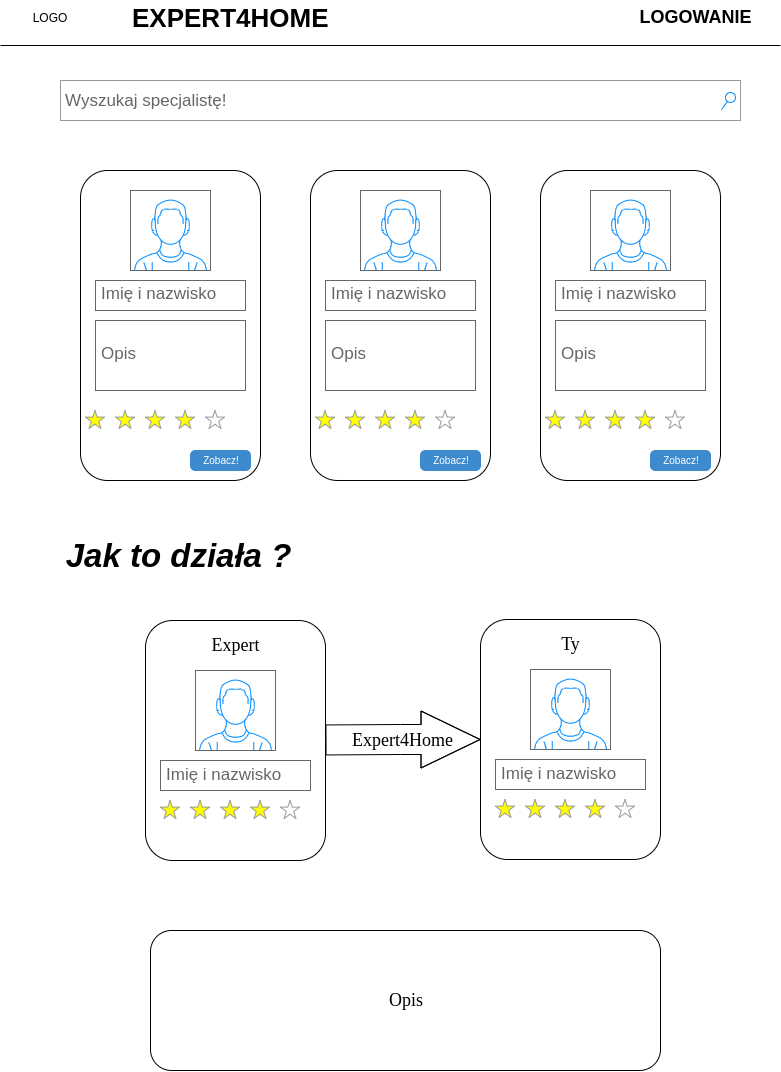
\includegraphics{Home view.png}

	\subsection{Ekran wyszukiwania specjalisty}

		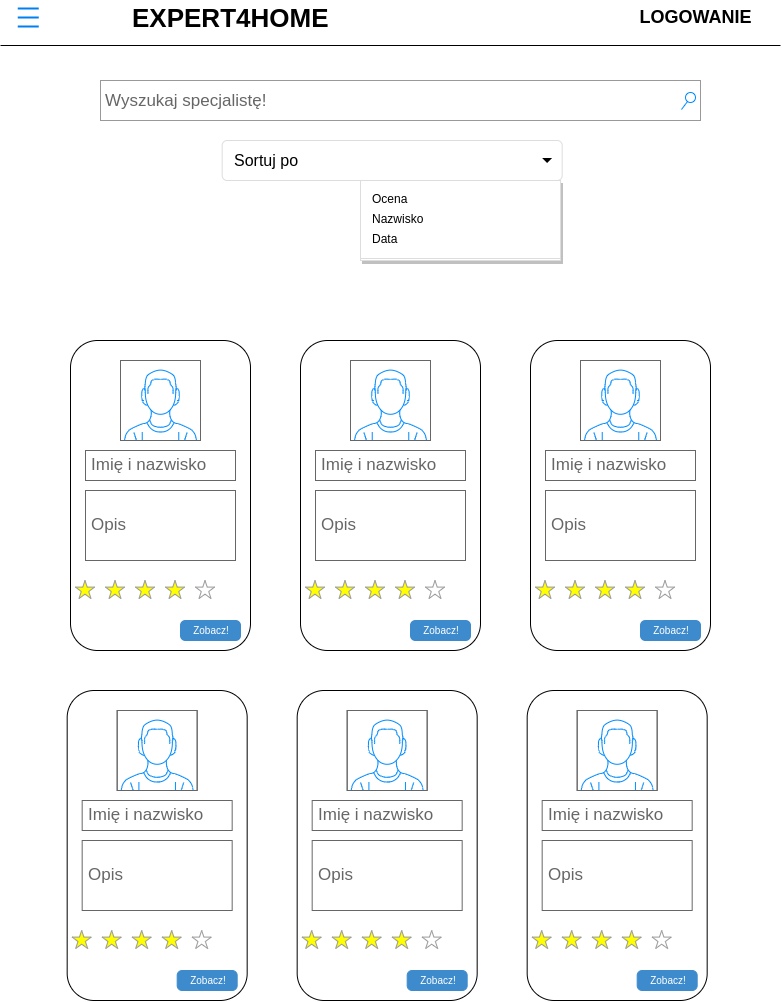
\includegraphics{Search expert view.png}

	\subsection{Ekran profilu specjalisty}	

		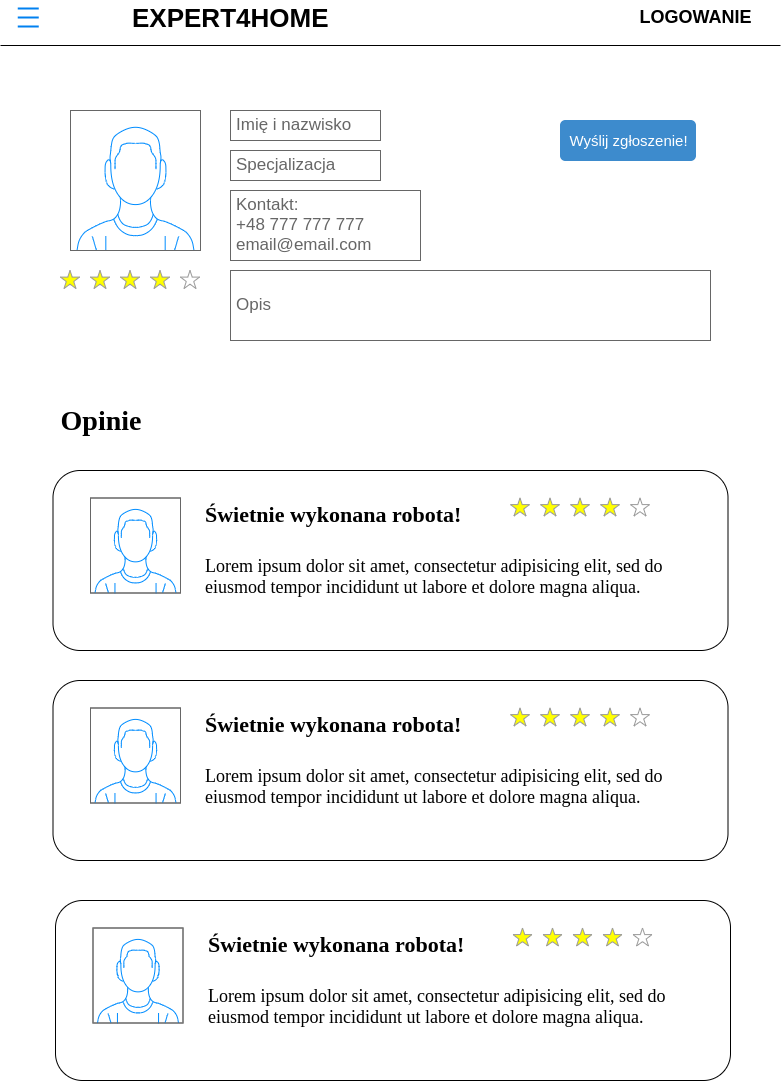
\includegraphics{Expert profile view.png}	
	
	\subsection{Dialog zgłoszenia}	
	todo sk przerysować w \url{https://draw.io} ze slackowego hash tag frontend, zapisać projekt do schemes, wyeksportować obraz do images, wstawić obraz tutaj z podpisem	
	
	\subsection{Ekran zgłoszeń klienta}
	todo sk przerysować w \url{https://draw.io} ze slackowego hash tag frontend, zapisać projekt do schemes, wyeksportować obraz do images, wstawić obraz tutaj z podpisem
	
	\subsection{Ekran zgłoszeń specjalisty}
	todo sk przerysować w \url{https://draw.io} ze slackowego hash tag frontend, zapisać projekt do schemes, wyeksportować obraz do images, wstawić obraz tutaj z podpisem  
  
	\section{Szczegóły implementacji}  
  
	\subsection{Środowisko deweloperskie}  
	Jednym z ważniejszych wyzwań jest zapewnienie spójności środowisk pomiędzy uczestnikami zespołu. Wszelkie
	nawet najmniejsze odchylenia mogą prowadzić do błędów, co gorsza większość problemów może być nie możliwa
	do odtworzenia na innych maszynach. Ponieważ wybraliśmy javę 8 jako język programowania niezbędna jest
	automatyzacja budowania oraz zarządzania zależnościami itp. Postanowiliśmy użyć programu gradle Gradle,
	posiada on prostą i przejrzystą składnie ułatwiającą pracę. Mimo ułatwienia jakim jest Gradle, nie jest
	wystarczającym środkiem zapewnienia spójności. W celu osiągnięcia jej postanowiliśmy skorzystać z
	kontenerów Dockerowych. Ze względu na rozmiar kontenerów Windowsowych, jedyną możliwą opcją są kontenery
	Linuxowe. Oznacza to iż platformą docelową dla każdego fragmentu aplikacji jest Alpine Linux. Konteneryzacja
	aplikacji ułatwia również późniejsze uruchomienie jej w środowisku chmurowym. Każdy z 3 najpopularniejszych
	dostawców oferuje hosting dla kontenerów.
  
	\subsection{Zastosowane technologie}

	\subsubsection{Front-end}	
	todo jg+sk react
	
	\subsubsection{Back-end}	
	% todo kd+km+pp springboot, mysql, nginx	
	Do serwerowej części projektu postanowiliśmy wykorzystać kilka technologii. Zostaną one opisane poniżej.
	  
	\paragraph{SpringBoot} \mbox{} \\
	Do napisania kodu części serwerowej aplikacji wybraliśmy framework \texttt{SpringBoot} języka \texttt{Java}.
	Jest to rozwiązanie sprawdzone przez wiele firm i rozwijane oraz wspierane już przez wiele lat. Dzięki temu możemy korzystać z dopracowanych bibliotek oraz zdobyć cenne doświadczenie.

	\texttt{SpringBoot} jest bazowany na frameworku \texttt{Spring} jednak w przeciwieństwie do niego znacznie ogranicza niepotrzebną konfigurację na rzecz konwencji.
	Dzięki takiemu podejściu programista może skupić się na realizowaniu funkcjonalności zamiast na przygotowywaniu środowiska.

	\paragraph{Tomcat} \mbox{} \\
	Do uruchomienia aplikacji oraz obsługi połączeń sieciowych zastosowany został serwer \texttt{Tomcat}.
	Jest to rozwiązanie o otwartym kodzie źródłowym wspierane przez organizację Apache.
	Stanowi domyślne rozwiązanie dla aplikacji sieciowych pisanych w języku Java.

	\paragraph{MySQL} \mbox{} \\
	Do przechowywania danych biznesowych aplikacji wybraliśmy bazę MySQL.
	Ponieważ dane maja wyraźną strukturę uznaliśmy, że rozwiązanie oparte na SQL będzie dobrze rozwiązywało problemy związane ze składowaniem danych.
	Baza \texttt{MySQL} posiada otwarty kod źródłowy, ma zaimplementowane wszystkie najważniejsze funkcjonalności silników bazodanowych takie jak transakcje, widoki czy wyzwalacze i jest to szeroko używane i sprawdzone rozwiązanie.

	\paragraph{Nginx} \mbox{} \\
	Przez wiele lat dominującym serwerem http na rynku był Apache. W 2019 został on zdetronizowany przez Nginxa. 
	Zdecydowaliśmy się użyć nowego króla. Głównych jego cechą jest możliwość obsługiwania bardzo dużej liczby
	połączeń jednocześnie, dzięki asynchronicznemu podejściu do obsługi zapytań. Apache obsługuje połączenia
	synchronicznie, tj. tworzy nowy proces dla każdego połączenia. Ponad to składnia konfiguracji Nginx jest
	znacznie bardziej przejrzysta niż konfiguracja Apache. Dodatkową zaletą Nginxa jest jego popularność. Oznacza
	to iż w sytuacji natrafienia na trudności istnieje duża szansa iż ktoś już kiedyś natrafił na podobny problem.
	
	\subsubsection{Kontrola wersji}
	todo bz git
	  
	\subsubsection{Wdrożenie oprogramowania}
	Istnienie kontenerów Dockerowy otwiera przed naszym zespołem wiele nowych możliwości. Dzięki sposobowi dystrybucji
	jakim jest Docker Hub w bardzo prosty sposób można uzyskać dostęp do wielu jż stworzonych obrazów dysków. Możliwym
	jest również rozstawienie własnego rejestru obrazów. W efekcie pobieranie wszelkiego rodzaju zależności sprowadza
	się do jednej komendy, gdzie każda zależności "myśli" że jest oddzielnym systemem operacyjnym. Przykładowo,
	jeżeli potrzebujemy bazy postgreSQL wystarczy wywołać komendę \texttt{docker pull postgres}, odpowiedni obraz
	zostanie pobrany.
	
	Docelowo środowiskiem produkcyjnym aplikacji będzie chmura Microsoft Azure. Dokładnie oferowany przez MSA hosting
	kontenerów. Zdecydowaliśmy się na Azure ze względu na możliwość połączenia ponieważ korzystamy z pakietu Azure DevOps. 
	Azure Devops pozwala na zarządzanie zadaniami, hostowanie prywatnych rejestrów Dockerowych oraz co najważniejsze,
	pozwala na definiowanie procesów CI/CD. W odpowiednim etapie dojrzałości projektu planujemy skorzystać z właśnie
	tej funkcjonalności w celu usprawnienia całego procesu wytwarzania oprogramowania.

	  
	\subsection{Plan testów}
	todo km jednostkowe, integracyjne, sam wiesz lepiej
 
	\section{Szczegóły organizacji prac}  
 
	\subsection{Harmonogram prac}
	todo bz
 
	\subsection{Metodyka wytwarzania oprogramowania}
	todo sk scrum, kanban
	
	\subsection{Zastosowane narzędzia}
	todo kd azure devops, slack
 
\end{document}